%%%%%%%%%%%%%%%%%%%%%%%%%%%%%%%%%%%%%%%%%%%%%%%%%%%%%%%%%%%%%%%%%%%%%
%% This is a (brief) model paper using the achemso class
%% The document class accepts keyval options, which should include
%% the target journal and optionally the manuscript type. 
%%%%%%%%%%%%%%%%%%%%%%%%%%%%%%%%%%%%%%%%%%%%%%%%%%%%%%%%%%%%%%%%%%%%%
\documentclass[journal=jacsat,manuscript=article]{achemso}

%%%%%%%%%%%%%%%%%%%%%%%%%%%%%%%%%%%%%%%%%%%%%%%%%%%%%%%%%%%%%%%%%%%%%
%% Place any additional packages needed here.  Only include packages
%% which are essential, to avoid problems later. Do NOT use any
%% packages which require e-TeX (for example etoolbox): the e-TeX
%% extensions are not currently available on the ACS conversion
%% servers.
%%%%%%%%%%%%%%%%%%%%%%%%%%%%%%%%%%%%%%%%%%%%%%%%%%%%%%%%%%%%%%%%%%%%%
\usepackage[version=3]{mhchem} % Formula subscripts using \ce{}

%%%%%%%%%%%%%%%%%%%%%%%%%%%%%%%%%%%%%%%%%%%%%%%%%%%%%%%%%%%%%%%%%%%%%
%% If issues arise when submitting your manuscript, you may want to
%% un-comment the next line.  This provides information on the
%% version of every file you have used.
%%%%%%%%%%%%%%%%%%%%%%%%%%%%%%%%%%%%%%%%%%%%%%%%%%%%%%%%%%%%%%%%%%%%%
%%\listfiles

%%%%%%%%%%%%%%%%%%%%%%%%%%%%%%%%%%%%%%%%%%%%%%%%%%%%%%%%%%%%%%%%%%%%%
%% Place any additional macros here.  Please use \newcommand* where
%% possible, and avoid layout-changing macros (which are not used
%% when typesetting).
%%%%%%%%%%%%%%%%%%%%%%%%%%%%%%%%%%%%%%%%%%%%%%%%%%%%%%%%%%%%%%%%%%%%%
\newcommand*\YE[1]{Ye: \texttt{\textbf{#1}}}

%%\newcommand{\YE}[1]{\textcolor{blue}{#1}}

%%%%%%%%%%%%%%%%%%%%%%%%%%%%%%%%%%%%%%%%%%%%%%%%%%%%%%%%%%%%%%%%%%%%%
%% Meta-data block
%% ---------------
%% Each author should be given as a separate \author command.
%%
%% Corresponding authors should have an e-mail given after the author
%% name as an \email command. Phone and fax numbers can be given
%% using \phone and \fax, respectively; this information is optional.
%%
%% The affiliation of authors is given after the authors; each
%% \affiliation command applies to all preceding authors not already
%% assigned an affiliation.
%%
%% The affiliation takes an option argument for the short name.  This
%% will typically be something like "University of Somewhere".
%%
%% The \altaffiliation macro should be used for new address, etc.
%% On the other hand, \alsoaffiliation is used on a per author basis
%% when authors are associated with multiple institutions.
%%%%%%%%%%%%%%%%%%%%%%%%%%%%%%%%%%%%%%%%%%%%%%%%%%%%%%%%%%%%%%%%%%%%%
\author{Ye Ding}
\affiliation{Atombeat Technology Pte. Ltd., 6 Rafflesr Quay, Singapore.}
\email{ye.ding@atombeat.com}
\author{Xinyan Wang}
\affiliation{Atombeat Technology Pte. Ltd., 6 Rafflesr Quay, Singapore.}
\email{xinyan.wang@atombeat.com}
\author{Rongfeng Zou}
\affiliation{Atombeat Technology Pte. Ltd., 6 Rafflesr Quay, Singapore.}
\author{Hang Zheng}
\affiliation{Atombeat Technology Pte. Ltd., 6 Rafflesr Quay, Singapore.}
\email{hzheng@atombeat.com}
%%%%%%%%%%%%%%%%%%%%%%%%%%%%%%%%%%%%%%%%%%%%%%%%%%%%%%%%%%%%%%%%%%%%%
%% The document title should be given as usual. Some journals require
%% a running title from the author: this should be supplied as an
%% optional argument to \title.
%%%%%%%%%%%%%%%%%%%%%%%%%%%%%%%%%%%%%%%%%%%%%%%%%%%%%%%%%%%%%%%%%%%%%
\title[An \textsf{achemso} demo]
  {Improving binding free energy predictions with Swap Monte Carlo for water sampling}

%%%%%%%%%%%%%%%%%%%%%%%%%%%%%%%%%%%%%%%%%%%%%%%%%%%%%%%%%%%%%%%%%%%%%
%% Some journals require a list of abbreviations or keywords to be
%% supplied. These should be set up here, and will be printed after
%% the title and author information, if needed.
%%%%%%%%%%%%%%%%%%%%%%%%%%%%%%%%%%%%%%%%%%%%%%%%%%%%%%%%%%%%%%%%%%%%%
\abbreviations{Free Energy Perturbation, Binding Free Energy, Monte Carlo, Water Sampling, Molecular Dynamics}
\keywords{American Chemical Society, \LaTeX}

%%%%%%%%%%%%%%%%%%%%%%%%%%%%%%%%%%%%%%%%%%%%%%%%%%%%%%%%%%%%%%%%%%%%%
%% The manuscript does not need to include \maketitle, which is
%% executed automatically.
%%%%%%%%%%%%%%%%%%%%%%%%%%%%%%%%%%%%%%%%%%%%%%%%%%%%%%%%%%%%%%%%%%%%%
\begin{document}

%%%%%%%%%%%%%%%%%%%%%%%%%%%%%%%%%%%%%%%%%%%%%%%%%%%%%%%%%%%%%%%%%%%%%
%% The "tocentry" environment can be used to create an entry for the
%% graphical table of contents. It is given here as some journals
%% require that it is printed as part of the abstract page. It will
%% be automatically moved as appropriate.
%%%%%%%%%%%%%%%%%%%%%%%%%%%%%%%%%%%%%%%%%%%%%%%%%%%%%%%%%%%%%%%%%%%%%
%\begin{tocentry}

%Some journals require a graphical entry for the Table of Contents.
%This should be laid out ``print ready'' so that the sizing of the
%text is correct.

%Inside the \texttt{tocentry} environment, the font used is Helvetica
%8\,pt, as required by \emph{Journal of the American Chemical
%Society}.

%The surrounding frame is 9\,cm by 3.5\,cm, which is the maximum
%permitted for  \emph{Journal of the American Chemical Society}
%graphical table of content entries. The box will not resize if the
%content is too big: instead it will overflow the edge of the box.

%This box and the associated title will always be printed on a
%separate page at the end of the document.

%\end{tocentry}

%%%%%%%%%%%%%%%%%%%%%%%%%%%%%%%%%%%%%%%%%%%%%%%%%%%%%%%%%%%%%%%%%%%%%
%% The abstract environment will automatically gobble the contents
%% if an abstract is not used by the target journal.
%%%%%%%%%%%%%%%%%%%%%%%%%%%%%%%%%%%%%%%%%%%%%%%%%%%%%%%%%%%%%%%%%%%%%
\begin{abstract}
Water molecules within and around the binding cavity can significantly influence the binding affinity of ligands. 
Proper sampling of these water molecules ensures that their contributions to the free energy landscape are accurately accounted for. 
In the pursuit of more accurate binding free energy calculations, we have developed a novel Swap Monte Carlo (SwapMC) method specifically designed for cavity water sampling. 
The SwapMC method aims to enhance the sampling efficiency by facilitating the movement of water molecules in and out of the protein cavity, thereby ensuring a comprehensive exploration of water distributions. 
By leveraging GPU power to perform Monte Carlo moves for water molecules in parallel across multiple sites, and integrating SwapMC with NPT simulations within the Uni-FEP framework, 
we have observed significant improvements in the accuracy of relative binding free energy calculations, all while maintaining computational efficiency. 
Our results demonstrate that SwapMC achieves performance comparable to Grand Canonical Monte Carlo (GCMC) methods in water-related test cases, offering a robust and efficient alternative for addressing the challenges associated with cavity water sampling in computational chemistry. 
%Furthermore, we have extended the SwapMC scheme to sample the distribution of ions in DNA/RNA simulations, 
%broadening the applicability of this method to a wider range of biomolecular systems and enhancing the accuracy of ion-related free energy calculations.
\end{abstract}

%%%%%%%%%%%%%%%%%%%%%%%%%%%%%%%%%%%%%%%%%%%%%%%%%%%%%%%%%%%%%%%%%%%%%
%% Start the main part of the manuscript here.
%%%%%%%%%%%%%%%%%%%%%%%%%%%%%%%%%%%%%%%%%%%%%%%%%%%%%%%%%%%%%%%%%%%%%
\section{Introduction}
Binding free energy calculation for protein-ligand interactions is an important tool in computational chemistry and drug discovery.
Mostly, the binding free energy calculations are performed with the free energy perturbation (FEP) method~\cite{jiang2010free, wang2019protein, Qian2024}.
FEP method employed molecular dynamics (MD) simulation to sample the conformational space of the system.
Through the perturbation of the ligand in different states, the binding free energy can be calculated with the statistical mechanics.
Accuracy of the binding free energy calculations is strongly dependent on the force field parameters~\cite{Ding2023, 17c36m, lu2021opls4, he2022recent, vanommeslaeghe2012automationI, vanommeslaeghe2012automationII} 
and the conformational sampling~\cite{15rex, wang2011replica, hritz2008hamiltonian} of the system.\\
\newline
The relative binding free energy (RBFE) calculations are consisted of a series of alchemical transformations, 
where the ligand is transformed from one state to another in the binding site of the protein.
And absolute binding free energy (ABFE) calculations are performed by decoupling the ligand from the protein cavity.
In both cases, the binding free energy calculations are sensitive to the conformational sampling of the system.
Alchemically changed states often involve the rearrangement of the binding site, 
which can lead to significant changes in the water distribution in the binding site.
Especially for the water molecules that are buried in the binding sites,
sampling these water molecules required a thorough exploration of the conformational space~\cite{zhou2009theory, cozzini2004free,li2007water}, 
which is a time consuming task in the MD simulations. \\
\newline
To address the challenges of water sampling in the binding site during the MD simulations,
multiple strategies have been proposed to enhance the sampling of water molecules~\cite{Wagle2024,ross2020enhancing,Ge2022,ben2021fast,Deng2024,Liu2025}.
The most common approach is to use the Grand Canonical Monte Carlo (GCMC) method~\cite{ross2015water, ross2020enhancing, Aldeghi2018, Bodnarchuk2014, deng2008computation, Samways2020, Woo2004}.
GCMC is a statistical mechanics method that allows for the insertion and deletion of water molecules in the binding site during the simulation.
There is also an extended way of GCMC, the Grand Canonical Non-equilibrium candidate Molecular Dynamics (GCNCMD)~\cite{Bergazin2020,Ge2022,melling2023enhanced,Deng2024}.
These methods have shown significant improvements in the accuracy of binding free energy calculations.
Besides, there are also some other methods that can predict the water's distribution in the binding site for a fast equilibration, 
such as the Grid Inhomogeneous Solvation Theory (GIST)~\cite{Abel2008,Michel2009,Cao2019,Irwin2019,Eberhardt2023} and the hybrid MC/MD method proposed by Ben-Shalom et.al~\cite{BenShalom2019,ben2021fast}.
But these methods are often computationally expensive and complex to implement. 
Most MD engines do not support these methods natively~\cite{Samways2020,Cezar2020,Nejahi2021,Nejahi2019}, which makes them less accessible for routine use in binding free energy calculations.
Besides, the chemical potential in GCMC is often difficult to set up and requires careful tuning for different time steps and water models~\cite{deng2008computation,ross2020enhancing}.\\
\newline
In this work, we present a novel Swap Monte Carlo (SwapMC) method designed to efficiently sample water molecules in the cavity during binding free energy calculations.
SwapMC is a Monte Carlo-based method that allows for the exchange of water molecules in and out of the protein cavity during the simulation.
The method is implemented in the Uni-FEP framework within the OpenMM~\cite{Eastman2023} simulation engine.
By combining the SwapMC method with the NPT ensemble, we can efficiently sample the water molecules in the binding site without the need for complex GCMC implementations.
SwapMC avoids the need for setting up the chemical potential with it's compatibility with the NPT ensemble.
Furthermore, with the parallelization run on GPUs, SwapMC can perform the Monte Carlo moves for water molecules in parallel across multiple sites, 
that improved the sampling efficiency and reduced the computational cost. \\
\newline
We begin by describing the SwapMC workflow in Uni-FEP framework, 
and discussed the how the detailed balance is satisfied in the SwapMC method.
The acceptance ratio is derived from the detailed balance condition.
Then, we present the performance of SwapMC in binding free energy calculations on the water sets in Gregory's work~\cite{ross2020enhancing}.
The water's density distribution in the protein cavity is also analyzed to demonstrate the effectiveness of SwapMC in sampling water molecules.
Finally, we compare the performance of SwapMC with GCMC in binding free energy calculations,
and show that SwapMC achieves comparable performance with GCMC in the same test cases.
\section{Method}
\subsection{Workflow of the Swap Monte Carlo}
SwapMC was designed to exchange water molecules in and out of the protein cavity during FEP calculations, Fig.~\ref{fig:scheme} A.
Unlike the rectangular region that defined in Ben-Shalom's work~\cite{ben2021fast}, 
the cavity region in our protocol is represented by a spherical space that centered at the geometric center of the ligand coordinates, $R^{in}$ in Fig.~\ref{fig:scheme} B.
The radius is half the maximum intra-atomic distance within the ligands, plus an additional 0.3 nanometers for buffer.
All other areas of the simulation box are considered outside this spherical cavity and will be referred to $R^{out}$ space hereafter, Fig.~\ref{fig:scheme} B.
Thus, the SwapMC algorithm workflow consists of these steps:
\begin{enumerate}
  \item Randomly decide the exchange direction, ensuring an equal chance of moving water in or out of the cavity.
  \item A water molecule $i$ is chosen for deletion from the source region with the probability defined in Eq.~\ref{eq:selection_probability}. Where $u_i$ represents the interaction energy of water molecule $i$ with other atoms in the simulation box. $N_{src}$ denotes the number of exchangeable water molecules in the source region. A higher $u_i$ increases the likelihood of a molecule being selected. 
  \begin{equation}\label{eq:selection_probability}
    p_i = \frac{e^{u_i}}{\sum^{N_{src}}_k{e^{u_k}}}    
  \end{equation}
  \item Uniform sampling the potential insertion sites over the destination region.
  \item The combination of the sampled sites with 60 orientations of water molecule results in 18,000 possible insertion conformations.
  \item Evaluate the interaction energy for each of the 18,000 water molecules in the simulated system, denoted as $u_j$.
  \item Sequentially iterate over the potential insertion conformation, and calculate the acceptance ratio $A_{S_i \to S_j}$ using $u_i$ and $u_j$, determine if the conformation is acceptable. 
  If it is, terminate this iteration.
  \item Replace the deleted water positions by the accepted conformation coordinates and set this water molecule's velocity to zero for the simulation stability.
\end{enumerate}

\begin{figure}
  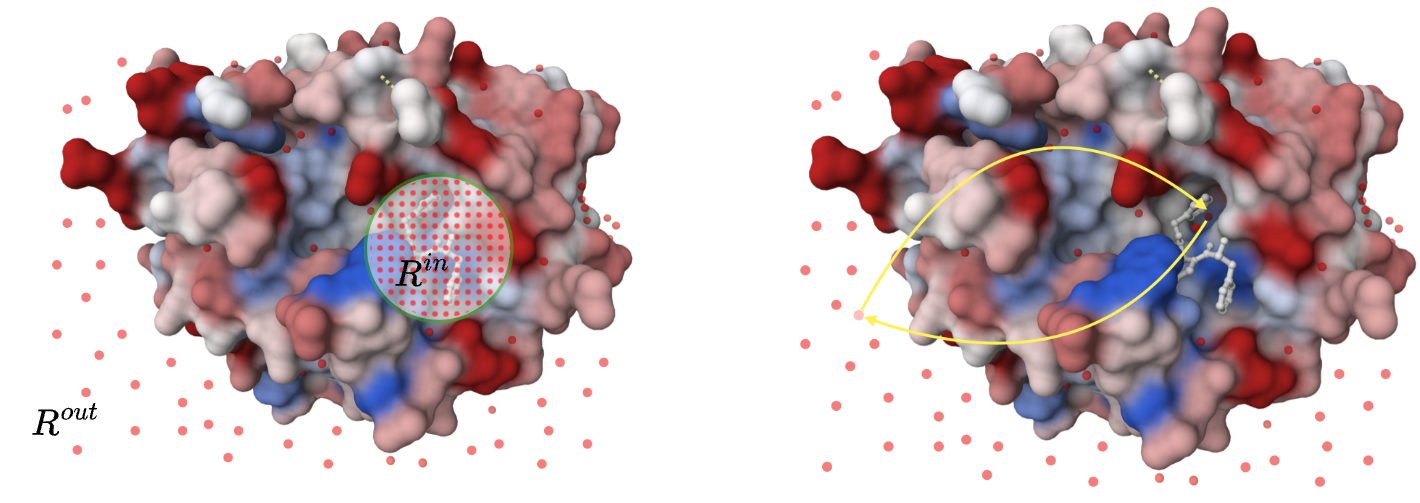
\includegraphics[width=0.9\textwidth]{figures/SwapMonteCarlo-scheme.png}
  \caption{Schematic Figure for Swap Monte Carlo (SwapMC) Method.
  The figure illustrates the process of moving water molecules in and out of the protein cavity during simulation.}
  \label{fig:scheme}
\end{figure}

\subsection{Detailed Balance in Swap Monte Carlo}
In the Monte Carlo algorithm, the acceptance ratio $A_{S_i \to S_j}$ between two states $S_i$ and $S_j$ must satisfy detailed balance:
\begin{equation}\label{eq:acceptance_ratio}
\frac{A_{S_i \to S_j}}{A_{S_j \to S_i}}=\frac{G_{S_j \to S_i} P_{S_j}}{G_{S_i \to S_j} P_{S_i}}
\end{equation}
\noindent Where $P_{S_j}$ and $P_{S_i}$ represent the equilibrium probabilities of states $S_j$ and $S_i$, respectively. 
The terms $G_{S_i \to S_j}$ and $G_{S_j \to S_i}$ denote the transition probabilities for the transformation from state $S_i$ to state $S_j$, and vice versa.
As the Metropolis criteria indicated, in simulations, the acceptance ratio $A_{S_i \to S_j}$ for the transformation from state $S_i$ to $S_j$, is defined as:
\begin{equation}\label{eq:metropolis}
A_{S_i \to S_j}=\min \left\{1, \frac{G_{S_j \to S_i} P_{S_j}}{G_{S_i \to S_j} P_{S_i}}\right\}
\end{equation} \\
\newline
In the context of Swap Monte Carlo, state $S_i$ represent the water molecule located in position $\mathbf{x}_i$, and state $S_j$ represents the water molecule located in position $\mathbf{x}_j$, where the other atoms remains fixed.
Thus, the equilibrium probabilities $P_{S_i}$ and $P_{S_j}$ followed a Boltzmann distribution in the grand canonical ensemble, expressed as:
\begin{equation}\label{eq:equilibrium_probability}
  \begin{aligned}
  P_{S_i}\left(\mathbf{x}_1, \ldots, \mathbf{x}_i, \ldots\mathbf{x}_n\right) & \propto \frac{e^{n B}}{n!} e^{-\beta U\left(\mathbf{x}_1, \ldots, \mathbf{x}_i,\ldots, \mathbf{x}_n\right)}  \\
  P_{S_j}\left(\mathbf{x}_1, \ldots, \mathbf{x}_j, \ldots\mathbf{x}_n\right) & \propto \frac{e^{n B}}{n!} e^{-\beta U\left(\mathbf{x}_1, \ldots, \mathbf{x}_j,\ldots, \mathbf{x}_n\right)}
  \end{aligned}
\end{equation} 
Where $U\left(\mathbf{x}_1, \ldots, \mathbf{x}_i,\ldots, \mathbf{x}_n\right), U\left(\mathbf{x}_1, \ldots, \mathbf{x}_j,\ldots, \mathbf{x}_n\right)$ denotes the potential energy of the states $S_i, S_j$, 
$\beta = \frac{1}{kT}$ is the inverse temperature, $k$ is the Boltzmann constant, and $n$ is the number of particles in the system.
A fundamental relationship emerges from the potential energy difference between two states $S_i$ and $S_j$:
\begin{equation}\label{eq:potential_energy_interaction}
U\left(\mathbf{x}_1, \ldots, \mathbf{x}_j,\ldots, \mathbf{x}_n\right) - U\left(\mathbf{x}_1, \ldots, \mathbf{x}_i,\ldots, \mathbf{x}_n\right) = u_j - u_i
\end{equation}
Where $u_i$ and $u_j$ are the interaction energies of the moved water molecule in states $S_i$ and $S_j$, respectively.
\newline
The transition probability matrix element $G_{S_i \to S_j}$ quantifies the likelihood of transitioning from state $S_i$ to state $S_j$. 
Given the statistical independence between molecular deletion and insertion events, 
the composite transition probability necessarily factorizes as:
\begin{equation}\label{eq:transition_probability_decomposition}
G_{S_i \to S_j} = g_{S_i}^{(\text{del})} \cdot g_{S_j}^{(\text{ins})}
\end{equation}
Where $g_{S_i}^{(\text{del})}$ and $g_{S_j}^{(\text{ins})}$ represent the respective marginal probabilities for water molecule removal from state $S_i$ and insertion into state $S_j$.
With the previous workflow steps, the deletion probability $g_{S_i}^{(\text{del})}$ is defined as the probability of selecting a water molecule $i$ for deletion from the source region, 
given by Eq.~\ref{eq:selection_probability}, 
and the insertion probability $g_{S_j}^{(\text{ins})}$ is defined as the uniform sampling of the potential insertion sites over the destination region.
Thus, the transformation probability matrix elements $G_{S_i \to S_j}$ and $G_{S_j \to S_i}$ can be expressed as:
\begin{equation}\label{eq:transition_probability}
  \begin{aligned}
G_{S_i \to S_j} &= p_i \cdot \frac{1}{V_{S_j}} = \frac{e^{u_i}}{\sum^{N^{S_i}_{src}}_k{e^{u_k}}} \cdot \frac{1}{V_{S_j}} \\
G_{S_j \to S_i} &= p_j \cdot \frac{1}{V_{S_i}} = \frac{e^{u_j}}{\sum^{N^{S_j}_{src}}_k{e^{u_k}}} \cdot \frac{1}{V_{S_i}}  
  \end{aligned}
\end{equation}
Where $V_{S_i}$ and $V_{S_j}$ denote the volume of the source region in states $S_i$ and $S_j$, respectively.
The source region cardinalities $N_{\text{src}}^{S_i}$ and $N_{\text{src}}^{S_j}$ in the transition probability elements $G_{S_i \to S_j}$ and $G_{S_j \to S_i}$ correspond to distinct spatial domains within the simulation framework, 
as their respective source regions differ between the transformation $S_i \to S_j$ and $S_j \to S_i$.
Assume the position $\mathbf{x}_i$ is within the cavity region $R^{in}$, and the position $\mathbf{x}_j$ is outside the cavity region $R^{out}$.
The source region $N_{\text{src}}^{S_i}$ is defined as the set of water molecules within the cavity region $R^{in}$, 
and the source region $N_{\text{src}}^{S_j}$ is defined as the set of water molecules outside the cavity region $R^{out}$ plus the moved water molecule in position $\textbf{x}_j$. \\
%To formally distinguish these non-overlapping regions, we employ the notation $N_{\text{src}}^{S_i}$ and $N_{\text{src}}^{S_j}$ as domain-specific particle counts.
\newline
By substitute the components in Eq.~\ref{eq:metropolis} with the Eq.~\ref{eq:equilibrium_probability},~\ref{eq:potential_energy_interaction},~\ref{eq:transition_probability},
we obtained the acceptance criterion for the exchange of water molecules in transition $S_i \to S_j$:
\begin{equation}\label{eq:acceptance_criterion}
A_{S_i \to S_j} = \min \left\{1, \frac{V_{S_j}}{V_{S_i}} \cdot \frac{\sum^{N^{S_i}_{src}}_k{e^{u_k}}}{\sum^{N^{S_j}_{src}}_k{e^{u_k}}} \right\}
\end{equation}
\noindent The acceptance criterion required the calculations on the interaction energies $u_k$ of all water molecules in the source region $N^{S_i}_{src}$ or $N^{S_j}_{src}$,
which can be efficiently performed in parallel on GPUs.
\subsection{Implementation of Swap Monte Carlo in Uni-FEP}
To implement the SwapMC method in the Uni-FEP framework, we have rewritten the non-bonded interaction module in OpenMM to support the efficient calculation of interaction energies for water molecules in the simulation box.
Besides, we have also implemented the interaction energy calculation for the inserted water molecules in the potential insertion sites.
The evaluation of the interaction energy for each of the 18,000 water molecules in the simulated system is performed in parallel on GPUs,
allowing for efficient computation of the acceptance ratio $A_{S_i \to S_j}$ for each potential insertion conformation.
The implementation of SwapMC is designed to be compatible with the existing Uni-FEP framework, 
without loss of MD simulation performance.
%\YE{We need to add the performance comparison with NPT here.}

\section{Results}
For a robust validation of the Swap Monte Carlo method, 
we conducted a series of tests to evaluate its performance in free energy calculations.
Gregory et.al~\cite{ross2020enhancing} performed a comprehensive evaluation of the GCMC method for water sampling in the RBFE calculations.
The test set in Gregory's work includes 94 ligands in 8 diverse protein-ligand systems.
For each system, the transformation of the ligands in RBFE calculations is related to the water displacement in the protein cavity.
GCMC has been shown to be effective in sampling water molecules in the protein cavity~\cite{ross2015water},
and showed a significant improvement in the accuracy of RBFE calculations compared to the traditional MD simulations for RBFE with water displacement transformation.
In this work, we made a direct comparison of the performance of SwapMC with GCMC in the same test cases.
All tests were performed with the Uni-FEP framework.
RBFE simulations were performed with the Uni-FEP framework, 
each replica was run for 5~\textit{ns} with a time step of 4~\textit{fs}.
SwapMC was performed every 500 steps (2~\textit{ps}) during the simulation.
300 potential insertion sites were uniformly sampled in the cavity region for each replica.
TIP3P~\cite{Jorgensen1983} water model was used in all simulations.
Ligands parameterization was performed with GAFF2~\cite{he2020fast} and ff14SB~\cite{Maier2015} was used for protein force field.


\subsection{Water Sampling in Protein Cavity}
For a more intuitive understanding of the water displacement in the protein cavity, 
we have selected two ligands from the HSP90 protein-ligand system, Ligand 9 and Ligand 7, as shown in Fig.~\ref{fig:hsp90} A.
The transformation of Ligand 9 to Ligand 7 involves the core hopping change of the two ligands,
which results in a subtle water distribution change in the protein cavity.
However, the change of the water distribution in the cavity is hard to be captured by the traditional MD simulations.
Especially for the structures without pre-equilibration, the water molecules in the cavity region are not well sampled.\\
\newline
In the test, we performed the alchemical transformation of Ligand 9 to Ligand 7.
The water molecules in the cavity region were removed in the input structure of the simulation.
Fig.~\ref{fig:hsp90} B showed changes of the number of contact water molecules.
Number of contact water molecules is defined as the number of water molecules that are within 5~\textit{Å} from the heavy atoms of the alchemical changed group of the ligands.
In the cavity region with different replicas during the alchemical transformation.
Within the 5~\textit{ns} simulation for each replica,
the number of contact water molecules with SwapMC is significantly higher than that without SwapMC.
Ligand 7 has larger number of contact water molecules in the cavity region than Ligand 9,
which is consistent with the ligand structure change.
These results indicate that SwapMC made a more thorough sampling of the water molecules in the cavity region.
And it also captured the subtle change of the water distribution in the cavity region with distinct ligands.
With the SwapMC enabled, the RBFE results for the alchemical transformation of Ligand 9 to Ligand 7 is significantly improved 4.59~\textit{kcal/mol} compared to the results without SwapMC.
\begin{figure}
  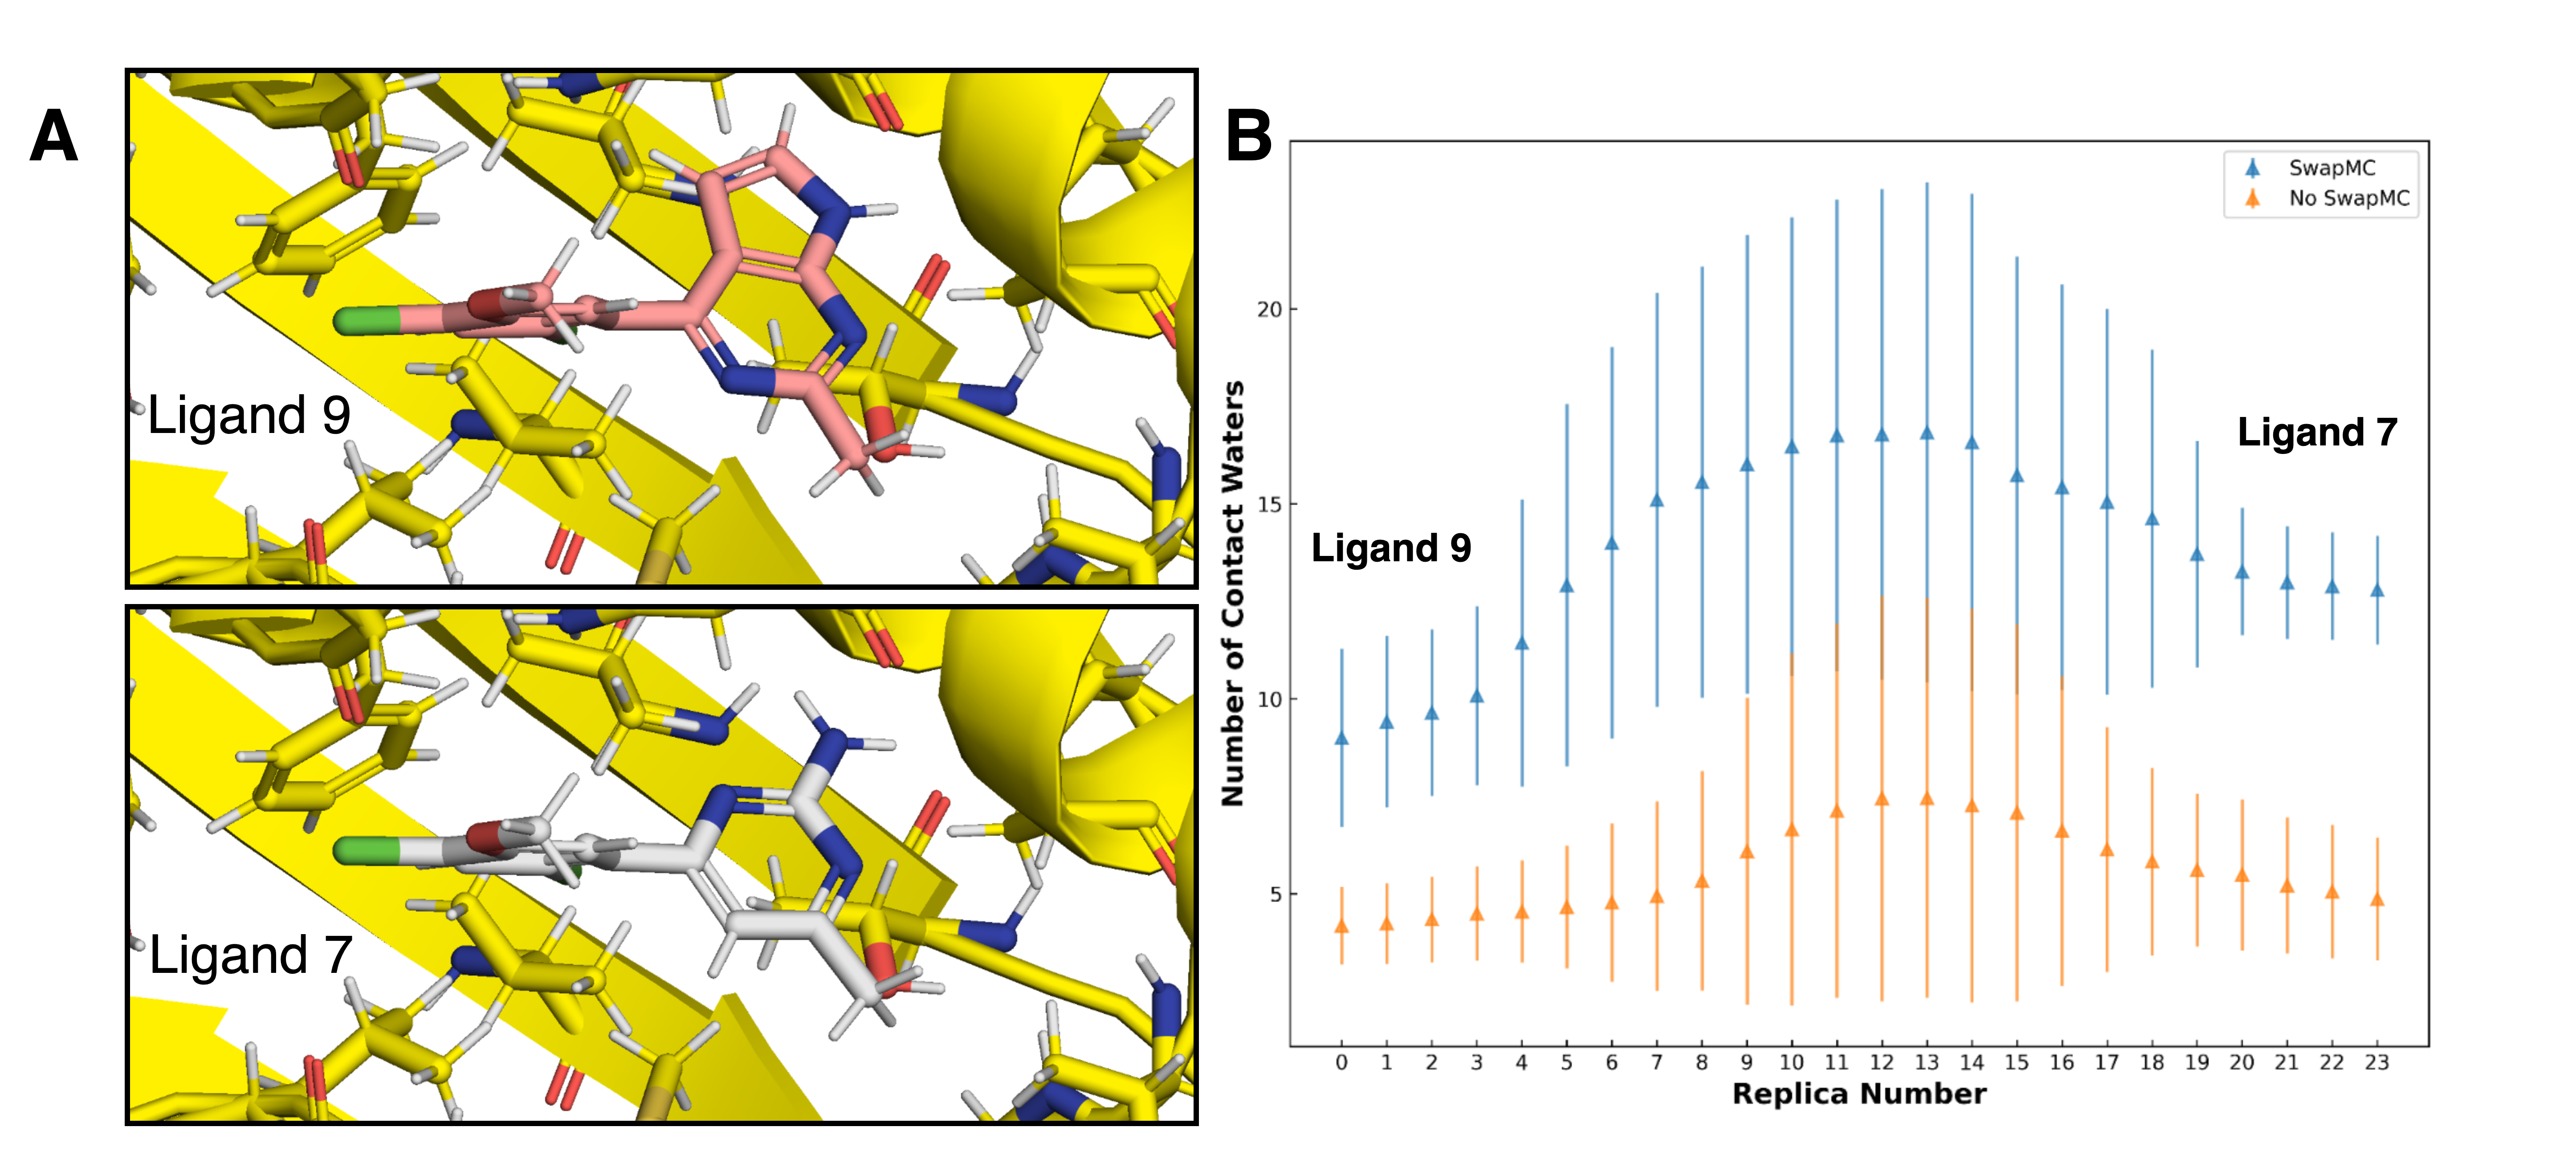
\includegraphics[width=0.9\textwidth]{figures/hsp90.png}
  \caption{Water sampling in the HSP90 protein cavity in the presence of a ligand. 
  Panel A shows the two ligands (Ligand 9 and Ligand 7) used in the test.
  Panel B shows the number of contact water molecules in the cavity region during the alchemical transformation of Ligand 9 to Ligand 7.
  Replica 0 denotes the Ligand 9 state, and Replica 23 denotes the Ligand 7 state.
  }
  \label{fig:hsp90}
\end{figure}

\subsection{Performance on RBFE Calculations}
Water sampling was significantly improved with the SwapMC method.
That paved the way for the RBFE calculations with water displacement transformation.
We have performed the RBFE calculations on the water sets in Gregory's work~\cite{ross2020enhancing}.
For a fair comparison, we conducted four sets of RBFE calculations for each system:
With and without SwapMC, and with and without cavity waters (CW.).
Cavity waters are the crystal waters that located in the 6~\textit{Å} radius of the ligand heavy atoms.
All simulations were ran with the same protocol as described in the previous section.\\ 
\newline
The RBFE results are shown in Table~\ref{tbl:rbfe_watersets}.
Compared to the results without SwapMC, the RBFE results with SwapMC show a significant improvement in accuracy.
Besides, SwapMC showed a good consistency in the RBFE results with and without cavity waters in input structure.
Which indicates the robustness of the SwapMC method in water sampling.
Furthermore, the RBFE results with SwapMC are comparable to the GCMC results in these systems.
These results demonstrate that SwapMC can be an effective alternative to GCMC for water sampling in RBFE calculations.

\begin{table}
  \caption{RBFE results for water sets, where CW denotes Cavity Waters. All edges correspond to those utilized in Gregory's study~\cite{ross2020enhancing}. 
  The ddG RMSE and $R^2$ values are computed using experimental binding free energies. 
  The unit of ddG RMSE is \textit{kcal/mol}, with $R^2$ presented in parentheses. 
  The optimal results are highlighted in \textbf{bold}.}
  \label{tbl:rbfe_watersets}
  \begin{tabular}{l|lllll}
    \hline
    System                    & No CW.     & No CW.        & With CW.    & With CW.     & GCMC by  \\
    ddG RMSE ($R^2$)          & No SwapMC  & With SwapMC   & No SwapMC   & With SwapMC  & Gregory et.al~\cite{ross2020enhancing} \\
    \hline
    Brd4(1)                      & 1.34 (0.67) & 0.87 (0.82) & 1.07 (0.71) & \textbf{0.64 (0.93)} & 1.74 (0.01) \\
    Chk1                         & 2.99 (0.02) & 1.67 (0.43) & 2.64 (0.10) & 1.70 (0.47) & \textbf{0.78 (0.80)} \\
    HSP90\_Kung                  & 3.85 (0.11) & 1.51 (0.59) & 3.90 (0.16) & \textbf{1.50} (0.50) & 2.14 (\textbf{0.62}) \\
    HSP90\_Woodhead              & 2.27 (0.83) & 0.61 (0.98) & 2.25 (0.84) & 0.65 (0.97) & \textbf{0.26} (\textbf{1.00}) \\
    Scytalone                    & 2.25 (0.73) & 1.45 (0.84) & 1.90 (0.80) & \textbf{1.39 (0.85)} & 1.86 (0.77) \\
    Taf1(2)                      & 2.01 (0.08) & 0.70 (0.51) & 0.76 (0.34) & 0.66 (0.51) & \textbf{0.66 (0.78)} \\
    Thrombin                     & 1.37 (0.34) & 1.14 (0.64) & 1.20 (0.46) & \textbf{1.13 (0.66)} & 1.15 (0.49) \\
    Urokinase                    & 0.74 (0.62) & 0.91 (0.36) & 0.81 (0.52) & 0.94 (0.32) & \textbf{0.70 (0.74)} \\
    \hline
  \end{tabular}
\end{table}

\subsection{Performance on ABFE Calculations}
The performance of SwapMC was also evaluated in the absolute binding free energy (ABFE) calculations.
During the ABFE calculations, the decoupling of the ligand from the protein cavity requires the water molecules in the cavity to be well sampled.
Reorganization of the water molecules in the cavity region is crucial for the accurate calculation of the binding free energy.
Previous studies~\cite{Liu2025} have shown that enhancing the sampling of water molecules in the cavity region can improve the convergence of the ABFE calculations. \\
\newline
In this work, we have performed the ABFE calculations on the JACS set and compared the performance of SwapMC with the results ordinary MD simulations.
The ABFE calculations were performed with the same protocol as described in the previous section.
The JACS set consists of 8 protein-ligand systems, and the binding free energy calculations were performed with the Uni-FEP framework.
The results are shown in Table~\ref{tbl:abfe_jacs}.
Compared to the results without SwapMC, the ABFE results with SwapMC show a significant improvement in the accuracy of the binding free energy calculations.
Most of the systems show a significant reduction in the dG RMSE, and the $R^2$ values are also improved.

\begin{table}
  \caption{ABFE Results for JACS set with and without SwapMC.}
  \label{tbl:abfe_jacs}
  \begin{tabular}{l|ll}
    \hline
    System                    & No SwapMC     & With SwapMC    \\
    dG RMSE ($R^2$)           &               &    \\
    \hline
    BACE                      & 3.27 (0.25) & 2.06 (0.36)  \\
    CDK2                      & 3.99 (0.09) & 3.73 (0.45)  \\
    JNK1                      & 2.01 (0.48) & 3.31 (0.50)  \\
    MCL1                      & 2.05 (0.34) & 1.94 (0.36)  \\
    P38                       & 3.22 (0.31) & 1.97 (0.48) \\
    PTP1B                     & 8.78 (0.29) & 7.16 (0.17) \\
    Thrombin                  & 1.67 (0.35) & 0.82 (0.68) \\
    TYK2                      & 2.51 (0.40) & 2.10 (0.43) \\
    \hline
  \end{tabular}
\end{table}


\section{Conclusion and Discussion}
We present a novel Swap Monte Carlo (SwapMC) method designed to efficiently sample water molecules in the cavity during binding free energy calculations.
Compared with the traditional MD simulations, SwapMC significantly improves the sampling of water molecules in the cavity region.
By integrating SwapMC with the Uni-FEP framework, the binding free energy calculations gained a notable improvements under the NPT ensemble.
Further testing on the water sets in Gregory's work~\cite{ross2020enhancing} demonstrated that SwapMC achieves comparable performance with GCMC in binding free energy calculations. 
Without the tuning of the chemical potential in SwapMC makes it it easy to be extended to other FEP framework. 
We hope that our work can provide a robust and efficient alternative for addressing the challenges associated with cavity water sampling in computational chemistry. \\
\newline
Currently, SwapMC was only implemented for the water molecules in the protein cavity.
Extend the SwapMC method to sample the distribution of ions in DNA/RNA simulations is a promising direction for future work.
Furthermore, monte carlo methods can also be applied to sample the distribution of other small molecules in the binding site,
such as the ligand fragments or the co-factors\cite{Cezar2020,goel2021rapid}.
This can further enhance the accuracy of the binding free energy calculations and broaden the applicability of SwapMC to a wider range of biomolecular systems.


%%%%%%%%%%%%%%%%%%%%%%%%%%%%%%%%%%%%%%%%%%%%%%%%%%%%%%%%%%%%%%%%%%%%%
%% The "Acknowledgement" section can be given in all manuscript
%% classes.  This should be given within the "acknowledgement"
%% environment, which will make the correct section or running title.
%%%%%%%%%%%%%%%%%%%%%%%%%%%%%%%%%%%%%%%%%%%%%%%%%%%%%%%%%%%%%%%%%%%%%
\begin{acknowledgement}
The author Ye Ding thanks Dr. Zilin Song, Prof. Jing Huang from Westlake University for their helpful discussions and suggestions on the SwapMC project.
\end{acknowledgement}

%%%%%%%%%%%%%%%%%%%%%%%%%%%%%%%%%%%%%%%%%%%%%%%%%%%%%%%%%%%%%%%%%%%%%
%% The same is true for Supporting Information, which should use the
%% suppinfo environment.
%%%%%%%%%%%%%%%%%%%%%%%%%%%%%%%%%%%%%%%%%%%%%%%%%%%%%%%%%%%%%%%%%%%%%
%\begin{suppinfo}

%This will usually read something like: ``Experimental procedures and
%characterization data for all new compounds. The class will
%automatically add a sentence pointing to the information on-line:

%\end{suppinfo}

%%%%%%%%%%%%%%%%%%%%%%%%%%%%%%%%%%%%%%%%%%%%%%%%%%%%%%%%%%%%%%%%%%%%%
%% The appropriate \bibliography command should be placed here.
%% Notice that the class file automatically sets \bibliographystyle
%% and also names the section correctly.
%%%%%%%%%%%%%%%%%%%%%%%%%%%%%%%%%%%%%%%%%%%%%%%%%%%%%%%%%%%%%%%%%%%%%
\bibliography{ref, common_ref}

\end{document}